%%%%%%%%%%%%%%%%%%%%%%%%%%%%%%%%%%%%%%%%%%%%
% https://github.com/martinhelso/uioposter %
%%%%%%%%%%%%%%%%%%%%%%%%%%%%%%%%%%%%%%%%%%%%
% Class options                            %
%%%%%%%%%%%%%%%%%%%%%%%%%%%%%%%%%%%%%%%%%%%%
% Orientation:                             %
% portrait (default), landscape            %
%                                          %
% Paper size:                              %
% a0paper (default), a1paper, a2paper,     %
% a3paper, a4paper, a5paper, a6paper       %
%                                          %
% Language:                                %
% english (default), norsk                 %
%%%%%%%%%%%%%%%%%%%%%%%%%%%%%%%%%%%%%%%%%%%%
\documentclass[a0paper]{uioposter}


\usepackage{lipsum}                                % Dummy text
\usepackage[figwidth = 0.98\linewidth]{todonotes}  % Dummy image (and more!)
\usepackage[absolute, overlay]{textpos}            % Figure placement
\usepackage{polyglossia}
\usepackage{graphicx}
\usepackage{qrcode}
\usepackage{xurl}
\usepackage{subcaption}
\usepackage{showframe}
\renewcommand\ShowFrameLinethickness{1.5pt}
\renewcommand*\ShowFrameColor{\color{red}}
\setmainlanguage{czech}
\setotherlanguages{english}
\usepackage[mono=true]{libertinus-otf}
\usepackage{microtype}
\setlength{\TPHorizModule}{\paperwidth}
\setlength{\TPVertModule}{\paperheight}


\title{Konceptuální modelování pomocí schematických kategorií}
\author{Dennis Pražák}
%% Optional:
\institute{prazak.dennis@gmail.com}
% Or:
%\institute{Contact information}


%% Remove footline:
%\setbeamertemplate{footline}{}

\begin{document}
\begin{frame}
  \begin{columns}[onlytextwidth]
    \begin{column}{0.5\textwidth - 1.5cm}
      \begin{block}{Úvod a motivace}
        \textbf{\alert{Konceptuální modely}} jako ER a UML byly vyvinuty v době, kdy měl největší zastoupení v databázových systémech jeden logický model, a to relační.
        V dnešní době se však kromě relačního modelu ve vyšší míře používá mnoho odlišných logických modelů (grafový, dokumentový, dvojice klíč/hodnota, sloupcový\dots).

        \textbf{\alert{Schematická kategorie}} je novým prostředekem ke konceptuálnímu modelování, který je obecnější (má vyšší vyjadřovací sílu) a není natolik provázaný s relačním modelem.
        Schematické kategorie splňují požadavky vyplývající z teorie kategorií, a lze na ně tak aplikovat již vybudované nástroje tohoto oboru matematiky.

        Cílem této práce bylo vytvořit webovou aplikaci, která umožní konceptuální modelování pomocí schematických kategorií v již známém modelu Entity-Relationship.
        Vytvořené ER schéma se automaticky převede na odpovídající schematickou kategorii.
        Usnadní tak výzkumníkům a potenciálním uživatelům schematických kategorií seznámení se s tímto novým konceptem.
      \end{block}

      \begin{block}{Příklad diagramů}
        \begin{figure}
          \centering
          \begin{subfigure}{0.45\textwidth}
            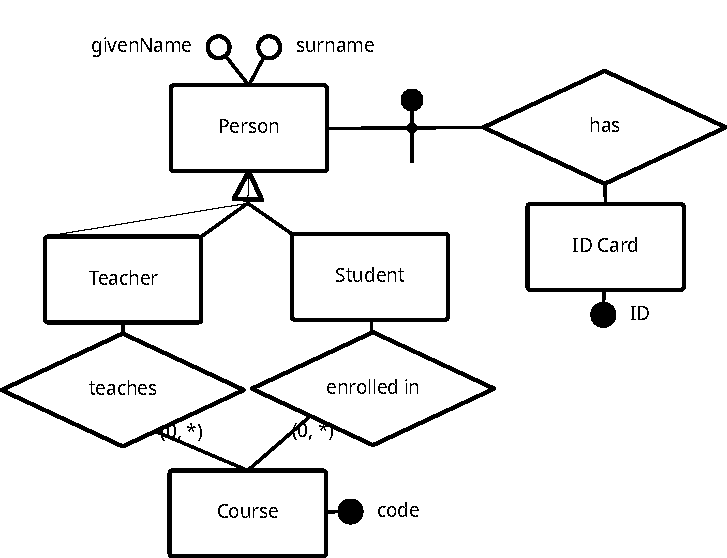
\includegraphics[width=1\textwidth]{./images/university-er.pdf}
            \caption*{ER schéma}
          \end{subfigure}
          \begin{subfigure}{0.45\textwidth}
            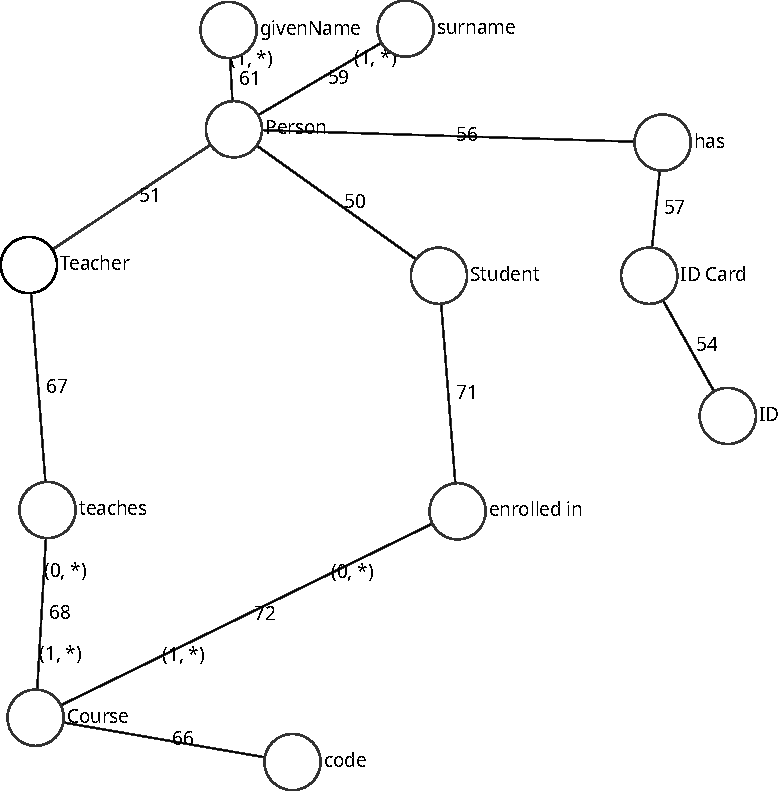
\includegraphics[width=\textwidth]{./images/university-schemcat.pdf}
            \caption*{Schematická kategorie}
          \end{subfigure}
          \begin{subfigure}{0.5\textwidth}
            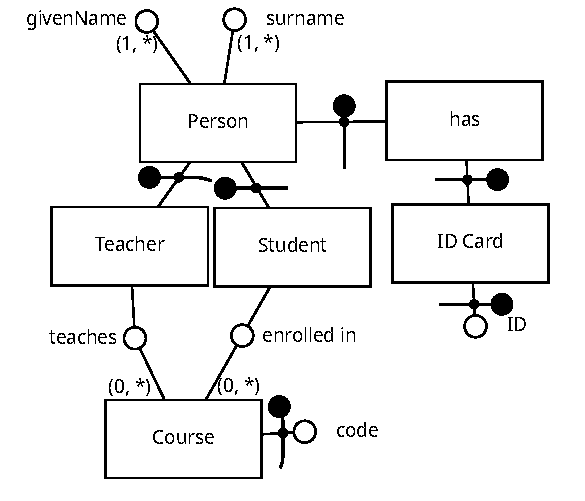
\includegraphics[width=\textwidth]{./images/university-scv.pdf}
            \caption*{Vizuální notace}
          \end{subfigure}
          %\caption{Diagramy}
        \end{figure}

        Na prvním obrázku je ER schéma vysoké školy s učiteli a studenty, kteří učí resp. docházejí na lekce.
        Na dalším obrázku lze vidět odpovídající schematickou kategorii.
        Záměrně zde kvůli zjednodušení nezobrazujeme všechny položky, které schematická kategorie obsahuje.
        Uživatel je může prozkoumat zvolením jednotlivých objektů nebo morfismů.
        Uživatelsky přívětivější podání schematické kategorie pak vidíme na posledním obrázku.
      \end{block}
    \end{column}


    \begin{column}{0.5\textwidth - 1.5cm}
      \begin{block}{Uživatelské rozhraní}
        \begin{figure}
          \centering
          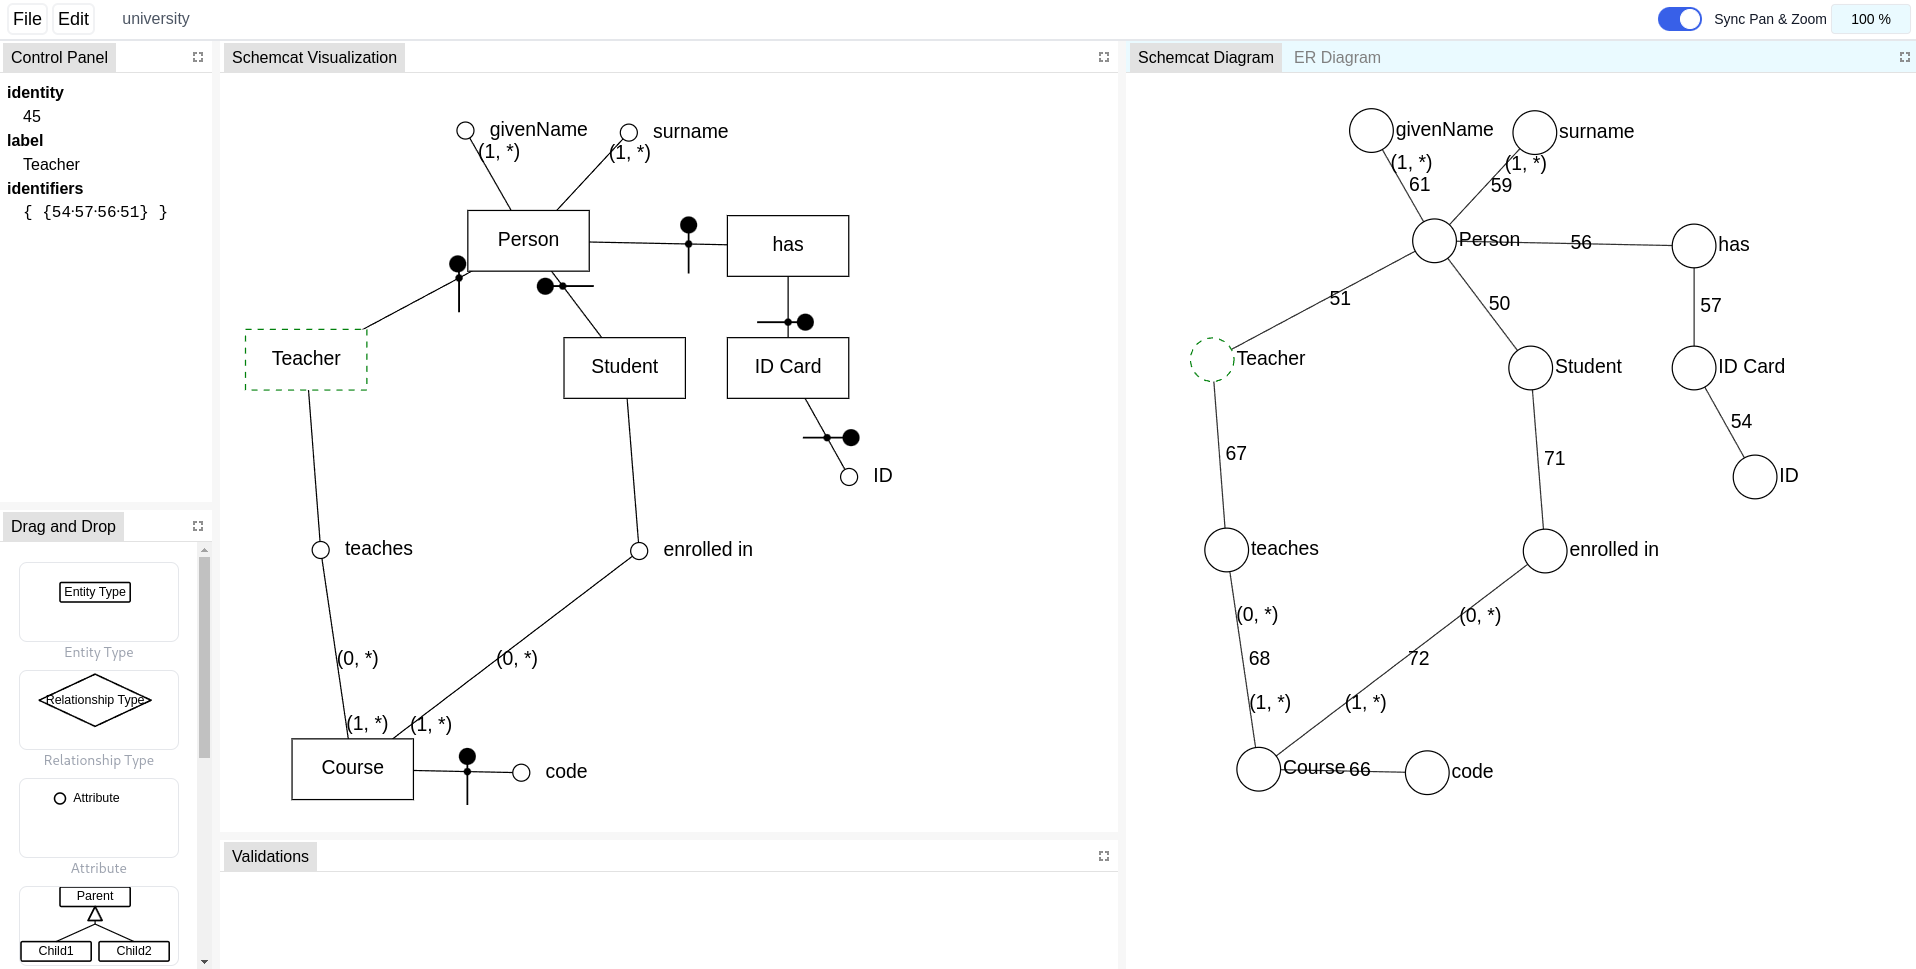
\includegraphics[width=0.8\textwidth]{./images/identifier-screenshot.png}
          \caption*{Uživatelské rozhraní}
          \label{fig:user-interface}
        \end{figure}

        Uživatelské rozhraní z Obrázku~\ref{fig:user-interface} je složeno z oken a záložek, které lze libovolně přesouvat a měnit jejich velikost.
        Na obrázku je právě zvolen objekt odpovídající entitnímu typu učitele a v ovládacím panelu vlevo lze vidět jeho jediný identifikátor 54$\cdot$57$\cdot$56$\cdot$51.
        To je řetězec složený ze signatur morfismů, které vedou do objektu, jímž je učitel identifikován (ID identifikační karty).

        Vlevo dole vidíme různé předpřipravené konstrukty (entitní typ, vztahový typ, atribut, ISA hierarchii, atd.), které lze přetažením myší vložit do ER diagramu.

        Dole je (prázdný) seznam validací, který potenciálně ukazuje některé detekované chyby v ER diagramu, které by způsobovaly, že diagram není validní (např.~existující cyklus slabé identifikace).
      \end{block}
      \begin{block}{Závěr}
        Webová aplikace byla dále navržena tak, aby umožnila potenciální rozšíření.
        Například:
        \begin{itemize}
          \item přímá tvorba a úprava schematických kategorií,
          \item online interaktivní spolupráce více uživatelů.
        \end{itemize}
      \end{block}
      \begin{block}{Odkazy}
        \begin{tabular}{rll}
          \qrcode[link,padding,hyperlink,height=5cm]{https://sorashi.github.io/schemcat}  & \href{https://sorashi.github.io/schemcat}{\texttt{sorashi.github.io/schemcat}}   & aplikace     \\
          \qrcode[link,padding,hyperlink,height=5cm]{https://github.com/sorashi/schemcat} & \href{https://github.com/sorashi/schemcat}{\texttt{github.com/sorashi/schemcat}} & zdrojový kód
        \end{tabular}
      \end{block}
    \end{column}
  \end{columns}


  \begin{textblock}{0.5}(0.63, 0.935)
    \color{white}
    \sffamily
    \begin{tabular}{rl}
      Vedoucí:    & RNDr.~Martin Svoboda,~PhD.
      \\
      Pracoviště: & Katedra softwarového inženýrství
    \end{tabular}
  \end{textblock}


\end{frame}
\end{document}
